\makeatletter
\def\beamer@framenotesbegin{% at beginning of slide
  \gdef\beamer@noteitems{}%
  \gdef\beamer@notes{{}}% used to be totally empty.
}
\makeatother
\setbeamertemplate{note page}{%
  \insertnote%
}

\usepackage{listings}
\lstset{basicstyle=\ttfamily\small}
\lstset{language=Python,
  stringstyle=\color{blue},
  commentstyle=\color{red},
  showstringspaces=false}
\lstdefinelanguage{APDL}{comment=[l]!}
\lstdefinelanguage{Abaqus}{comment=[l]**}
\usepackage{graphicx} \graphicspath{{content/figures/}}
\usepackage{booktabs}
\usepackage{cool}
\usepackage{bm} % bold math
\usepackage{siunitx}
\usepackage[backend=biber,natbib=true,style=authoryear,sorting=none,firstinits=true]{biblatex}
\addbibresource{content/cse_bibliography.bib}
\addbibresource{content/v2.bib}

%%% Macros for commonly-used symbols

% \ensuremath (from amsmath) so that we can use commands in regular text,
% or in math mode
% \xspace to ensure that we can easily write \DeltaK or \DeltaK-decreasing and
% not \DeltaK{} or \DeltaK{}-decreasing

\usepackage{xspace}

\newcommand{\hone}{\ensuremath{h_1}\xspace} % this is no shorter than $h_1$, but much easier to type overall. No, we can't use \h1 unless we define a command for \h that gobbles up the next block of text.
\newcommand{\htwo}{\ensuremath{h_2}\xspace}
\newcommand{\hthree}{\ensuremath{h_3}\xspace}
\newcommand{\hfour}{\ensuremath{h_4}\xspace}

\newcommand{\G}{\ensuremath{\bm{\mathcal{G}}}\xspace}
\newcommand{\Gc}{\ensuremath{\G_\textnormal{c}}\xspace} % G critical

\newcommand{\M}{\ensuremath{M}\xspace}

\newcommand{\K}{\ensuremath{K}\xspace}
\newcommand{\Kap}{\ensuremath{\K_\textnormal{ap}}\xspace} % K apparent
\newcommand{\Kef}{\ensuremath{\K_\textnormal{eff}}\xspace} % K effective
\newcommand{\Kel}{\ensuremath{\K_\textnormal{el}}\xspace} % K elastic
\newcommand{\Kpl}{\ensuremath{\K_\textnormal{pl}}\xspace} % K plastic
\newcommand{\Ktotal}{\ensuremath{\K_\textnormal{total}}\xspace} % K total
\newcommand{\Kr}{\ensuremath{\K_\textnormal{r}}\xspace} % K ratio
\newcommand{\Kmin}{\ensuremath{\K_\textnormal{min}}\xspace} % K min
\newcommand{\Kmax}{\ensuremath{\K_\textnormal{max}}\xspace} % K max
\newcommand{\DeltaK}{\ensuremath{\Delta \K}\xspace} % Delta K
\newcommand{\DeltaKth}{\ensuremath{\Delta \K_{\textnormal{th}}}\xspace} % K threshold
\newcommand{\KI}{\ensuremath{\K_\textnormal{I}}\xspace} % K mode I
\newcommand{\Kc}{\ensuremath{\K_\textnormal{c}}\xspace} % K critical
\newcommand{\KIc}{\ensuremath{\K_\textnormal{Ic}}\xspace} % K mode I critical
\newcommand{\Kapp}{\ensuremath{\K_\textnormal{app}}\xspace} % K apparent
\newcommand{\DeltaKeff}{\ensuremath{\Delta K_\textnormal{eff}}\xspace} % Delta J

\newcommand{\J}{\ensuremath{J}\xspace}
\newcommand{\Jel}{\ensuremath{\J_\textnormal{el}}\xspace} % J elastic
\newcommand{\Jpl}{\ensuremath{\J_\textnormal{pl}}\xspace} % J plastic
\newcommand{\Jtotal}{\ensuremath{\J_\textnormal{total}}\xspace} % J total
\newcommand{\DeltaJ}{\ensuremath{\Delta \J}\xspace} % Delta J
\newcommand{\Jmin}{\ensuremath{\J_\textnormal{min}}\xspace} % J min
\newcommand{\Jmax}{\ensuremath{\J_\textnormal{max}}\xspace} % J max
\newcommand{\DeltaJeff}{\ensuremath{\Delta J_\textnormal{eff}}\xspace} % Delta J effective

\newcommand{\etael}{\ensuremath{\eta_\textnormal{el}}\xspace}
\newcommand{\etapl}{\ensuremath{\eta_\textnormal{pl}}\xspace} % plastic work factor, through crack
\newcommand{\zetapl}{\ensuremath{\zeta_\textnormal{pl}}\xspace} % plastic work factor, surface crack
\newcommand{\Deltapl}{\ensuremath{\Delta_\textnormal{pl}}\xspace}
\newcommand{\Sij}{\ensuremath{S_{i,j}}\xspace}

\newcommand{\dadn}{\ensuremath{\frac{da}{dN}}\xspace}
\newcommand{\dadc}{\ensuremath{\frac{da}{dc}}\xspace}
\newcommand{\dcdn}{\ensuremath{\frac{dc}{dN}}\xspace}
\newcommand{\da}{\ensuremath{da}\xspace}
\newcommand{\dc}{\ensuremath{dc}\xspace}

\newcommand{\Rb}{\ensuremath{R_{\textnormal{b}}}\xspace}

\newcommand{\ry}{\ensuremath{r_{\textnormal{y}}}\xspace} % first-order estimate of plastic zone size
\newcommand{\rp}{\ensuremath{r_{\textnormal{p}}}\xspace} % second-order estimate of plastic zone size

\newcommand{\Pmin}{\ensuremath{P_\textnormal{min}}\xspace} % P min
\newcommand{\Pmax}{\ensuremath{P_\textnormal{max}}\xspace} % P max

\newcommand{\Sb}{\ensuremath{\sigma_{\textnormal{b}}}\xspace} % Stress in bending
\newcommand{\St}{\ensuremath{\sigma_{\textnormal{t}}}\xspace} % Stress in tension
\newcommand{\Sf}{\ensuremath{\sigma_{\textnormal{f}}}\xspace} % Stress at failure
\newcommand{\Smax}{\ensuremath{\sigma_{\textnormal{max}}}\xspace} % Stress at failure
\newcommand{\Sxx}{\ensuremath{\sigma_{xx}}\xspace} % Normal stress in x direction
\newcommand{\Syy}{\ensuremath{\sigma_{yy}}\xspace} % Normal stress in y direction
\newcommand{\Sxy}{\ensuremath{\tau_{xy}}\xspace} % Shear stress in x direction on y face
\newcommand{\Szz}{\ensuremath{\sigma_{zz}}\xspace} % Normal stress in z direction
\newcommand{\Sxz}{\ensuremath{\tau_{xz}}\xspace} % Shear stress in x direction on z face
\newcommand{\Syz}{\ensuremath{\tau_{yz}}\xspace} % Shear stress in y direction on z face
\newcommand{\Sone}{\ensuremath{\sigma_{1}}\xspace} % First principal stress
\newcommand{\Stwo}{\ensuremath{\sigma_{2}}\xspace} % Second principal stress
\newcommand{\Sthree}{\ensuremath{\sigma_{3}}\xspace} % Third principal stress
\newcommand{\Sys}{\ensuremath{\sigma_{\textnormal{ys}}}\xspace} % Yield strength in shear
\newcommand{\Sy}{\ensuremath{\sigma_{\textnormal{y}}}\xspace} % Yield strength in tension
\newcommand{\Sut}{\ensuremath{\sigma_{\textnormal{ut}}}\xspace} % Ultimate tensile strength
\newcommand{\Sc}{\ensuremath{\sigma_{\textnormal{c}}}\xspace} % Plastic collapse strength
\newcommand{\Sr}{\ensuremath{\sigma_{\textnormal{r}}}\xspace} % Stress at failure
\newcommand{\Szero}{\ensuremath{\sigma_{0}}\xspace} % Flow stress
\newcommand{\Sigij}{\ensuremath{\sigma_{ij}}\xspace}
\newcommand{\deltaij}{\ensuremath{\delta_{ij}}\xspace} % Kronecker delta

\newcommand{\Sinner}{\ensuremath{S_\textnormal{inner}}\xspace}
\newcommand{\Souter}{\ensuremath{S_\textnormal{outer}}\xspace}

\newcommand{\ac}{\ensuremath{a_{\textnormal{c}}}\xspace} % Flaw length critical
\newcommand{\aapp}{\ensuremath{a_{\textnormal{app}}}\xspace} % Flaw length apparent

\newcommand{\deltat}{\ensuremath{\delta_\textnormal{t}}\xspace} % CTOD

\newcommand{\kt}{\ensuremath{k_\textnormal{t}}\xspace} % Stress concentration

\newcommand{\T}{\ensuremath{T}\xspace} % T stress for two-parameter fracture
\newcommand{\Be}{\ensuremath{\beta}\xspace} % biaxiality ratio
\newcommand{\Q}{\ensuremath{Q}\xspace}

\author[Renfro, Allen, Wilson]{Michael W. Renfro\thanks{Tennessee Tech University} \and Phillip A. Allen\thanks{NASA Marshall Space Flight Center} \and Christopher D. Wilson\footnotemark[1]}

\title[Development of Automated Models for EP SC(B) Plates]{Development of Automated Model Generation and Analysis of Surface Cracked Plates in Bending for Interpolated Elastic-Plastic \J-integral Solutions}

\date{May 15, 2019}

% Set the colors and overall frame layout
\usetheme{Cookeville}%
% Allow captions on floats in presentations, but disable numbering, as not every float in
% the printed document will automatically show up in the presentation.
\setbeamertemplate{caption}{\insertcaption}%
\setbeamertemplate{caption label separator}{}%
% Beamer doesn't support chapters, only parts.
% The printed document won't use parts, only chapters.
\let\chapter\part%
% Show a mostly-blank separator page at the start of each part (chapter)
\AtBeginPart{%
\frame{\partpage}%
% Could add a ToC for the part in the frame here, but as you can see it all in
% the headers above the frame, doesn't seem worthwhile.
}%
% Disable part numbering on title pages for parts. https://tex.stackexchange.com/questions/183616/
\setbeamertemplate{part page}{%
\begin{beamercolorbox}[sep=8pt,center,wd=\textwidth]{part title}%
  \usebeamerfont{part title}\insertpart\par%
\end{beamercolorbox}%
}%


\newcommand{\linktopage}[2]{\structure{\hyperlink{Navigation#1}{#2}}}

\begin{document}

\begin{frame}[plain]
\maketitle
\note{
\vfill
}
\end{frame}

\begin{frame}[plain]
% Last-minute adjustments:
% - get titles and frame numbers for start of each chapter,
% - adjust the NavigationX numbers and titles below to match,
% - rebuild the presentation PDF.
\begin{itemize}
\item \linktopage{3}{Introduction} %\structure{\hyperlink{Navigation3}{Introduction}}
\item \linktopage{6}{Literature Review}
\item \linktopage{12}{Modeling Preparation for Research Tasks}
\item \linktopage{14}{Research Plan for Bending Models and Modified TASC Program}
\item \linktopage{22}{Results and Discussion}
\item \linktopage{31}{Conclusions and Recommendations for Future Work}
\item \linktopage{35}{Appendix}
\end{itemize}
\note{
\vfill
}
\end{frame}

\part{Introduction}

\begin{frame}
\begin{columns}
\begin{column}{0.45\textwidth}
\begin{itemize}
\item Constraint and stress states can get pretty involved.
\item Semi-elliptical surface cracks (SC01) are among the simplest part-through crack cases, and are the subject of ASTM E2899.
\item Handbook or curve-fit solutions exist for the other geometries, but only for linear elastic materials.
\item NASA's TASC program covers elastic-plastic surface cracks in tension, but {\bfseries not} in bending.
\end{itemize}
\end{column}
\begin{column}{0.45\textwidth}
\begin{figure}[tbp]
\centering
\includegraphics[width=\columnwidth]{nasgro-geometries}
\end{figure}
\end{column}
\end{columns}

\note{
\vfill
}
\end{frame}

\begin{frame}
Research goals
\begin{itemize}
\item High quality set of elastic-plastic finite element analysis results as a basis for curve-fit or handbook calculations
\item Modified TASC program for bending or tension analysis
\end{itemize}
\note{
\vfill
}
\end{frame}

\part{Literature Review}

\section{Consensus Bending Stress Intensity Solution}

\begin{frame}
\begin{columns}
\begin{column}{0.65\textwidth}
For a surface crack in bending, stress intensity at a given location:
\begin{align*}
\KI &= (
        H \sigma_\text{b} F_\text{b}
        ) \left(\frac{\pi a}{Z}\right)^{0.5} \\
\sigma_\text{b} &= \frac{6 M}{W t^2} \\
Z &= 1 + 1.464\left(\frac{a}{c}\right)^{1.65} \\
F_\text{b} &= \left[ M_1 + M_2 \left( \frac{a}{t} \right)^2 + M_3 \left( \frac{a}{t} \right)^4 \right] f_\phi f_\text{wb} g \\
\end{align*}
...plus another 12 equations, and that's just for linear elastic materials.
\end{column}
\begin{column}{0.3\textwidth}
\vbox to .8\textheight{ % https://tex.stackexchange.com/questions/15244/why-does-vfill-not-work-inside-a-beamer-column
\vfill

For surface cracks in tension, we need ``only'' 10 equations.

\vfill

No such curve fit exists for elastic-plastic materials.

\vfill}
\end{column}
\end{columns}
\note{
\vfill
}
\end{frame}

\section[Engineering Approaches for EP and FP Analysis of Surface Cracks]{Engineering Approaches for Elastic-Plastic and Fully-Plastic Analysis of Surface-Cracked Plates in Bending}

\subsection{ASTM E2899}

\begin{frame}
ASTM E2899: Standard Test Method for Measurement of Initiation Toughness in Surface Cracks Under Tension and Bending
\begin{columns}[b]
\begin{column}{0.45\textwidth}
\begin{figure}
\centering
\includegraphics[width=0.9\columnwidth]{sc-terminology-e2899-modified}
\caption{Test specimen and crack configurations}
\end{figure}
\end{column}
\begin{column}{0.45\textwidth}
\begin{figure}
\centering
\includegraphics[width=0.9\columnwidth]{astm-e2899-4point-bend}
\caption{Four-point bend test configuration}
\end{figure}
\end{column}
\end{columns}
\note{
\vfill
}
\end{frame}


\begin{frame}
\begin{itemize}
\item Starter crack machined into flat plate, fatigued to sharpen crack front
\item CMOD monitored as tension or bending load increased monotonically
\item Either specimen fails or start of stable crack tearing is detected
\item Location where crack growth occurs is recorded
\item Conditions classified as linear elastic, elastic-plastic, or fully-plastic
\item If LEFM or EPFM, calculate constraint from tables
\item If LEFM, calculate \K from series of provided equations
\item If EPFM, {\bfseries use nonlinear FEA} to calculate \J
\end{itemize}
\note{
\vfill
}
\end{frame}

\subsection{Tool for Analysis of Surface Cracks (TASC)}

\begin{frame}
\begin{columns}
\begin{column}{0.45\textwidth}
ASTM E2899 is unusual in its analysis requirements
\begin{itemize}
\item requires results of elastic-plastic finite element analysis
\item other standards require much simpler calculations or graphical constructions
\item NASA TASC program satisfies requirements, but only for tension
\end{itemize}
Mechanics of bending is more complex than for tension (constraint, crack closure)
\end{column}
\begin{column}{0.45\textwidth}
\begin{figure}
\centering
\includegraphics[width=\columnwidth]{tasc-original}
\caption{NASA TASC program}
\end{figure}
\end{column}
\end{columns}
\note{
\vfill
}
\end{frame}

\begin{frame}
TASC: interpolation code using database of 600 EPFM results for flat plates in tension
\begin{columns}
\begin{column}{0.45\textwidth}
\begin{figure}
\centering
\includegraphics[width=0.8\textwidth]{tasc-geometries}
\caption{20 normalized geometries:\\ \(0.2 \leq \frac{a}{c} \leq 1.0,\; 0.2 \leq \frac{a}{t} \leq 0.8\)}
\end{figure}
\end{column}
\begin{column}{0.45\textwidth}
\begin{figure}
\centering
\includegraphics[width=0.8\textwidth]{tasc-materials}
\caption{30 normalized materials:\\ \(100 \leq \frac{E}{S_{\text{ys}}} \leq 1000,\; 3 \leq n \leq 20\)}
\end{figure}
\end{column}
\end{columns}
\note{
\vfill
}
\end{frame}

\part{Modeling Preparation for Research Tasks%
\note{
\vfill}
}

%\section{Verification of Two TASC Cases}

%\subsection{Applying Procedure to a New Material Model (\(\frac{E}{\Sys}=150\))}

\begin{frame}
\begin{columns}
\begin{column}{0.4\textwidth}
Verification of two TASC cases, applying procedure to a new material (\(\frac{E}{\Sys}=150\))
\end{column}
\begin{column}{0.5\textwidth}
\begin{figure}[tbp]
\centering
\includegraphics[width=\columnwidth]{e100_150_200_verification}
\caption{\label{fig:e100_150_200_verification} Comparison of normalized FEA results, interpolated result, and TASC raw data}
\end{figure}
\end{column}
\end{columns}
\note{
\vfill
}
\end{frame}

\part{Research Plan for Bending Models and Modified TASC Program%
\note{
\vfill}
}

\section{Creating Plate Models}

\begin{frame}
\begin{center}
\(t = 1 \quad 0.2 \leq \frac{a}{c} \leq 1.0 \quad 0.2 \leq \frac{a}{t} \leq 0.8\) \\
\(W = 5 \max(c, t) \quad \Sinner = W \quad \Souter = 2W \quad L = 1.1 \Souter\)
\end{center}
\begin{columns}
\begin{column}{0.45\textwidth}
\begin{figure}
\centering
\includegraphics[width=\columnwidth]{bend_ac02_at08_E0100_n03}
\caption{\label{fig:bend_ac02_at08_E0100_n03} Plate model, \(\frac{a}{c}=0.2\), \(\frac{a}{t}=0.8\)}
\end{figure}
\end{column}
\begin{column}{0.45\textwidth}
\begin{figure}
\centering
\includegraphics[width=\columnwidth]{bend_ac10_at02_E0100_n03}
\caption{\label{fig:bend_ac10_at02_E0100_n03} Plate model, \(\frac{a}{c}=1.0\), \(\frac{a}{t}=0.2\)}
\end{figure}
\end{column}
\end{columns}
\note{
\vfill
}
\end{frame}

\section{Solving Plate Models, Optimizing Boundary Conditions}

\begin{frame}
\citet{allenwells2014} reported \(M = \frac{r_{\phi} \Sys}{\J} < 25\) for tension

\begin{columns}
\begin{column}{0.45\textwidth}
\begin{figure}[tbp]
\centering
\includegraphics[width=0.7\columnwidth]{min_M_hist}
\caption{Histogram of \(M\) results from TASC tension model database}
\end{figure}
\end{column}
\begin{column}{0.45\textwidth}
\begin{figure}[tbp]
\centering
\includegraphics[width=0.7\columnwidth]{J-CMOD-extrapolation}
\caption{\J-CMOD graph used for extrapolation}
\end{figure}
\end{column}
\end{columns}
\note{
\vfill
}
\end{frame}

\begin{frame}
\begin{columns}
\begin{column}{0.45\textwidth}
\begin{figure}[tbp]
\centering
\includegraphics[width=0.9\columnwidth]{J_CMOD_bend_ac02_at02_L1100_W0500_E0100_n03_wrp}
\caption{\(\frac{a}{c}=0.2\), \(\frac{a}{t}=0.2\), \(E=100\), \(n=3\)}
\end{figure}
\end{column}
\begin{column}{0.45\textwidth}
Adjust boundary conditions until
\begin{itemize}
\item slope of last 20\% of \J-CMOD curve is \(20\times\) larger than initial slope
\item slope of last 20\% of \J-CMOD curve is \(<10\%\) different than slope of previous 20\%
\end{itemize}
at \(\phi=\) \SI{30}{\SIUnitSymbolDegree}
\end{column}
\end{columns}
\note{
\vfill
}
\end{frame}

\begin{frame}
Displacement control for tension models makes optimization easier
\begin{columns}[t]
\begin{column}{0.45\textwidth}
\begin{figure}[tbp]
\centering
\includegraphics[width=0.9\columnwidth]{secant-1}
\caption{\label{fig:secant-1}Example stress-strain curve using linear plus power law (LPPL) formulation}
\end{figure}
\end{column}
\begin{column}{0.45\textwidth}
\begin{figure}[tbp]
\centering
\includegraphics[width=0.9\columnwidth]{secant-2}
\caption{\label{fig:secant-2}Transformed to find required strain level}
\end{figure}
\end{column}
\end{columns}
\note{
\vfill
}
\end{frame}

\begin{frame}
Load control for bending models makes optimization more difficult
\begin{columns}[t]
\begin{column}{0.45\textwidth}
\begin{figure}[tbp]
\centering
\includegraphics[width=0.9\columnwidth]{secant-3}
\caption{\label{fig:secant-3}Example stress-strain curve using LPPL formulation, transformed to stress-controlled}
\end{figure}
\end{column}
\begin{column}{0.45\textwidth}
\begin{figure}[tbp]
\centering
\includegraphics[width=0.9\columnwidth]{secant-4}
\caption{\label{fig:secant-4}Transformed to find required stress level}
\end{figure}
\end{column}
\end{columns}
\note{
\vfill
}
\end{frame}

\section{Verification and Validation}

\begin{frame}
\begin{columns}[t]
\begin{column}{0.45\textwidth}
Abaqus validation
\begin{figure}[tbp]
\centering
\includegraphics[width=0.8\columnwidth]{{abq_plate_ac02_at02}}
\caption{\label{fig:abq_plate_ac02_at02} Example Abaqus bending model from FEACrack}
\end{figure}
\end{column}
\begin{column}{0.45\textwidth}
\J convergence
\begin{figure}[tbp]
\centering
\includegraphics[width=\columnwidth]{contour_integral_regions_warp3d}
\caption{\label{fig:fem-j-domains} Elements used in WARP3D \J calculations}
\end{figure}
\end{column}
\end{columns}
\note{
\vfill
}
\end{frame}

\section{Updates to TASC}

\begin{frame}[fragile]
\begin{itemize}
\item Don't break anything already working for tension
\item Make a \verb|results_bending| database alongside the existing \verb|results| database for tension
\item Identify any equations only valid for tension models
\item Replace with conditionals checking for model type, then use tension or bending equations as required
\item Interpolation method should need no changes
\item Validate a load-CMOD curve against existing bending experimental data
\end{itemize}
\note{
\vfill
}
\end{frame}

\part{Results and Discussion \note{\vfill}}

\section{Improvements to Initial Bending Models}

\subsection{\J Convergence Study}

\begin{frame}
\begin{columns}
\begin{column}{0.45\textwidth}
\begin{figure}[tbp]
\centering
\includegraphics[width=\columnwidth]{{bend_ac02_at08_E0100_n20_wrp_J_converge_abs}}
\caption{Convergence of \J across 10 domains}
\end{figure}
\end{column}
\begin{column}{0.45\textwidth}
\begin{figure}[tbp]
\centering
\includegraphics[width=\columnwidth]{negative_J}
\caption{Anomalous \J convergence graph}
\end{figure}
\end{column}
\end{columns}
\note{
\vfill
}
\end{frame}

\subsection{Addition of Elastic Boundary at Crack Face}

\begin{frame}
Why is \J higher at \(\phi=90\) in some cases? What happens to plate deflection?
\begin{columns}
\begin{column}{0.45\textwidth}
\begin{figure}[tbp]
\centering
\includegraphics[width=\columnwidth]{step-01-zoomed}
\caption{First load step}
\end{figure}
\end{column}
\begin{column}{0.45\textwidth}
\begin{figure}[tbp]
\centering
\includegraphics[width=\columnwidth]{step-30-zoomed}
\caption{Last load step}
\end{figure}
\end{column}
\end{columns}
\note{
\vfill
}
\end{frame}

\begin{frame}
\begin{figure}[tbp]
\centering
\includegraphics[width=0.9\columnwidth]{left-step-30-10x-zoomed-before.png}
\includegraphics[width=0.9\columnwidth]{left-step-30-10x-zoomed-after.png}
\caption{Plate deflection before and after addition of elastic boundary}
\end{figure}
\note{
\vfill
}
\end{frame}

\begin{frame}
\begin{columns}
\begin{column}{0.45\columnwidth}
\begin{figure}[tbp]
\centering
\includegraphics[width=\columnwidth]{before-J_CMOD_bend_ac10_at08_L1100_W0500_E0100_n20_wrp}
\caption{Before addition of elastic boundary}
\end{figure}
\end{column}
\begin{column}{0.45\columnwidth}
\begin{figure}
\centering
\includegraphics[width=\columnwidth]{after-J_CMOD_bend_ac10_at08_L1100_W0500_E0100_n20_wrp}
\caption{After addition of elastic boundary}
\end{figure}
\end{column}
\end{columns}
\note{
\vfill
}
\end{frame}

\begin{frame}
\begin{columns}
\begin{column}{0.45\columnwidth}
\begin{figure}[tbp]
\centering
\includegraphics[width=\columnwidth]{negative_J}
\caption{Before addition of elastic boundary}
\end{figure}
\end{column}
\begin{column}{0.45\columnwidth}
\begin{figure}
\centering
\includegraphics[width=\columnwidth]{negative_J_corrected}
\caption{After addition of elastic boundary}
\end{figure}
\end{column}
\end{columns}
\note{
\vfill
}
\end{frame}

\section{Validation of Purpose-Built Model Results}

\begin{frame}
\begin{columns}
\begin{column}{0.45\textwidth}
\begin{figure}[tbp]
\centering
\includegraphics[width=\columnwidth]{exp_validation_mesh_zoomed}
\caption{Crack front mesh of purpose-built experimental validation model}
\end{figure}
\end{column}
\begin{column}{0.45\textwidth}
\begin{figure}[tbp]
\centering
\includegraphics[width=\columnwidth]{experimental-validation-load-cmod}
\caption{Comparison of predicted load and CMOD between purpose-built model and experiment}
\end{figure}
\end{column}
\end{columns}
\note{
\vfill
}
\end{frame}

\section{Validation of Modified TASC Output}

\begin{frame}
\begin{columns}
\begin{column}{0.45\textwidth}
\begin{figure}[tbp]
\centering
\includegraphics[width=0.8\columnwidth]{tasc-modified-ui} \vspace{1ex}
\includegraphics[width=0.8\columnwidth]{tasc-force-cmod-validation}
\caption{Modified TASC Program}
\end{figure}
\end{column}
\begin{column}{0.45\textwidth}
\begin{figure}[tbp]
\centering
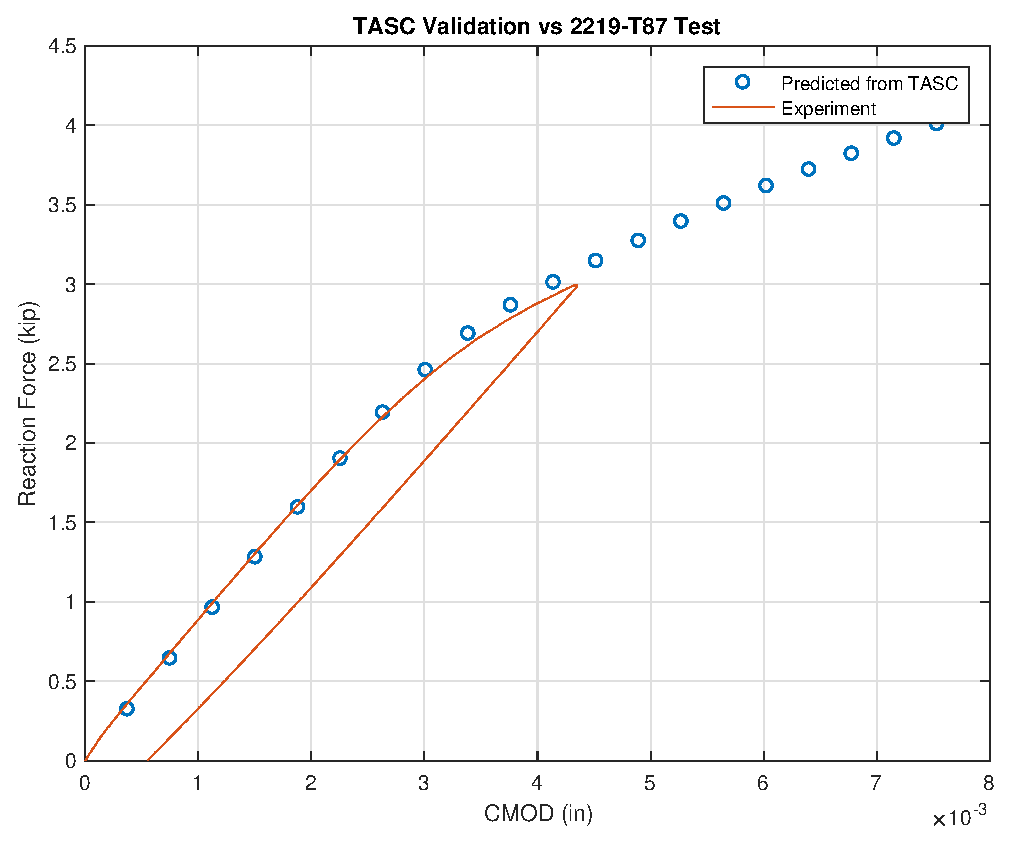
\includegraphics[width=0.75\columnwidth]{experimental-validation}
\caption{Comparison of TASC and experiment}
\end{figure}
\end{column}
\end{columns}
\note{
\vfill
}
\end{frame}

\section{Validation of \J Values between WARP3D and Abaqus}

\begin{frame}
\begin{columns}
\begin{column}{0.45\columnwidth}
\begin{figure}[tbp]
\centering
\includegraphics[width=\columnwidth]{{abq_bc_ac02_at02}}
\caption{Sample Abaqus validation model}
\end{figure}
\end{column}
\begin{column}{0.45\columnwidth}
\begin{figure}[tbp]
\centering
\includegraphics[width=\columnwidth]{{abq_wrp_ac02_at08_E1000_n20}}
\caption{Sample \J comparison between Abaqus and WARP3D}
\end{figure}
\end{column}
\end{columns}
\note{
\vfill
}
\end{frame}

\part{Conclusions and Recommendations for Future Work%
\note{\vfill}%
}

\section{Conclusions}

\begin{frame}
\begin{columns}
\begin{column}{0.6\textwidth}
%\begin{enumerate}
%\item
Database of 600 elastic-plastic finite element results for surface cracks in bending
\begin{itemize}
\item More challenging than tension models
\item Subset of results verified and validated against Abaqus and experimental data
\item Modified TASC program
\item Possible to satisfy requirements of ASTM E2899 for tension {\bfseries and} bending without constructing purpose-built EPFM models
\item Greatly reduces analytical burden on anyone doing ASTM E2899 tests
\end{itemize}
%\end{enumerate}
\end{column}
\begin{column}{0.3\textwidth}
\begin{figure}[tbp]
\centering
\includegraphics[width=0.8\columnwidth]{tasc-force-cmod-validation}
\end{figure}
\begin{figure}[tbp]
\centering
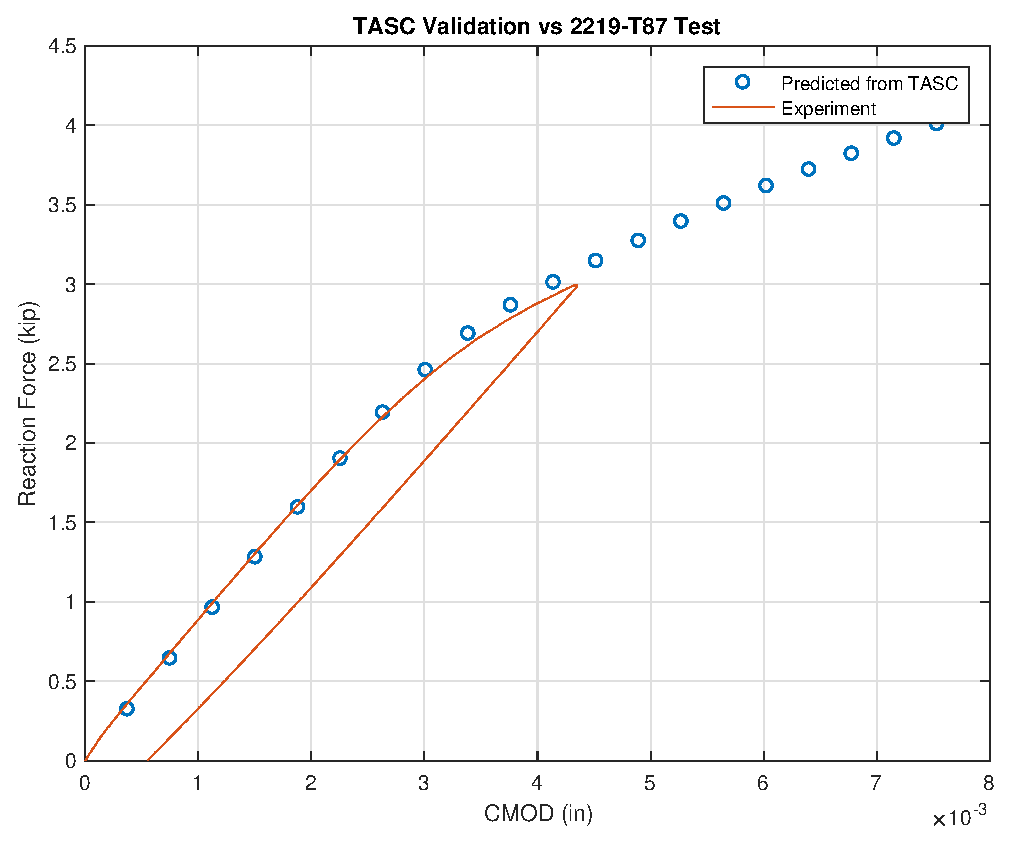
\includegraphics[width=0.75\columnwidth]{experimental-validation}
\end{figure}
\end{column}
\end{columns}
\note{
\vfill
}
\end{frame}

\section{Recommendations for Future Work}

\begin{frame}
\begin{enumerate}
\item TASC and E2899
\begin{itemize}
\item Finish integrating bend data into TASC, beyond load-CMOD validation
\item Additional values for material and/or crack geometry
\item Investigate other interpolation methods (piecewise cubic?)
\item Replace traction boundary conditions with rigid rollers and contact modeling
\end{itemize}
%\item EPRI \hone
%\begin{itemize}
%\item Further investigation into limits of \hone estimates
%\item Geometry, boundary conditions (types and magnitudes), materials
%\end{itemize}
%\item Load separation
%\begin{itemize}
%\item Alternative to R6 $\frac{b_\text{e}}{t}$ that drives \Sij to a single curve
%\end{itemize}
\item {\bfseries More experimental data needed for these.}
\end{enumerate}
\note{
\vfill
}
\end{frame}

\begin{frame}[plain]
\vfill
Thanks to:
\begin{itemize}
\item Tennessee Tech University's:
\begin{itemize}
\item Center for Manufacturing Research (Computer Aided Engineering)
\item Information Technology Services (High Performance Computing)
\end{itemize}
\item Quest Integrity's FEACrack
\item UIUC's WARP3D
\item Dassault's Abaqus
\item Anaconda's Python distribution
\end{itemize}
\vfill
\note{
\vfill
}
\end{frame}

\appendix

%\begin{frame}[plain]
% Last-minute adjustments:
% - get titles and frame numbers for start of each chapter,
% - adjust the NavigationX numbers and titles below to match,
% - rebuild the presentation PDF.
%\begin{itemize}
%\item \structure{\hyperlink{Navigation39}{Introduction to Fracture Mechanics}}
%\item \structure{\hyperlink{Navigation42}{Initial Verification of Quillen Models}}
%\item \linktopage{37}{Initial Verification of Two Tension Cases from \citet{allenwells2014}}
%\end{itemize}
%\end{frame}

\part{Initial Verification of Two Tension Cases from \citet{allenwells2014}}

\section{Extracting Normalized Results from the TASC Database}

\begin{frame}
\begin{columns}
\begin{column}{0.45\textwidth}
\begin{figure}[tbp]
\centering
\includegraphics[width=0.7\columnwidth]{aspect-ratio-gap}
\caption{\label{fig:aspect-ratio-gap} Gap in results for widest aspect ratios}
\end{figure}
\end{column}
\begin{column}{0.45\textwidth}
\begin{figure}[tbp]
\centering
\includegraphics[width=0.7\columnwidth]{modulus-gap}
\caption{Gap in results for lowest \(E\) values}
\end{figure}
\end{column}
\end{columns}
\end{frame}

\begin{frame}
\begin{columns}
\begin{column}{0.45\textwidth}
\begin{figure}[bp]
\centering
\includegraphics[width=\columnwidth]{tasc-inputs}
\caption{\label{fig:tasc_fea_inputs} Raw FEA results used in TASC}
\end{figure}
\end{column}
\begin{column}{0.45\textwidth}
\begin{figure}[tbp]
\centering
\includegraphics[width=\columnwidth]{tasc-results}
\caption{\label{fig:tasc_interp_outputs} Interpolated FEA results displayed by TASC}
\end{figure}
\end{column}
\end{columns}
\end{frame}

\section{Reconstructing Model Geometry in FEACrack}

\begin{frame}
\begin{columns}
\begin{column}{0.45\textwidth}
\begin{figure}[tbp]
\centering
\includegraphics[width=\columnwidth]{mesh-iso}
\caption{\label{fig:mesh-iso} Isometric view of overall mesh}
\end{figure}
\end{column}
\begin{column}{0.45\textwidth}
\begin{figure}[tbp]
\centering
\includegraphics[width=\columnwidth]{mesh-front}
\caption{\label{fig:mesh-front} Detailed view of crack front}
\end{figure}
\end{column}
\end{columns}
\end{frame}

\section{Reconstructing Material Parameters in FEACrack}

\begin{frame}

\begin{columns}
\begin{column}{0.45\textwidth}
\begin{align*}
\frac{\epsilon}{\epsilon_\text{ys}} &= 
\begin{cases}
\begin{aligned} % https://tex.stackexchange.com/a/385172
\hspace*{0.77em} \dfrac{\sigma}{\Sys} &,\enskip \epsilon \leq \epsilon_\text{ys} \\
\left(\dfrac{\sigma}{\Sys}\right)^{n} &,\enskip \epsilon > \epsilon_\text{ys}
\end{aligned}
\end{cases}
\end{align*}
where \(\epsilon_\text{ys} = \frac{\Sys}{E}\).
\end{column}
\begin{column}{0.45\textwidth}
\begin{figure}[tbp]
\centering
\includegraphics[width=\columnwidth]{lppl}
\caption{\label{fig:lppl} Set of LPPL stress-strain curves}
\end{figure}
\end{column}
\end{columns}

\end{frame}

\section{Applying Appropriate Boundary Conditions in FEACrack}

\begin{frame}
\begin{align*}
M &= \frac{r_\phi \Sys}{\J}
\end{align*}
\begin{table}[pb]
\caption{\label{tab:displacement_values} Applied displacement values for verification models}
\centering
\begin{tabular}{S[table-format=3.0] S[table-format=1.4] S *2{S[table-format=1.4]}} \toprule
{\(\frac{E}{\Sys}\)} & {Displacement} & {\(\phi\)} & {\(M\) using \(r_{\phi a}\)} & {\(M\) using \(r_{\phi b}\)} \\ \midrule
100 & 0.1028 & \SI{30}{\degree} & 15.9833 & 36.4241 \\
    &        & \SI{90}{\degree} & 22.6234 & 15.0822 \\
200 & 0.0550 & \SI{30}{\degree} & 24.7288 & 56.3542 \\
    &        & \SI{90}{\degree} & 34.9604 & 23.3069 \\
\bottomrule
\end{tabular}
\end{table}
\end{frame}

\section{Solving Models in WARP3D}

\begin{frame}
\begin{itemize}
\item 30 load steps
\item {\ttfamily warp3d < file.inp > file.out}
\item 21.6 minutes to solve on laptop, 2.2 minutes on HPC node
\end{itemize}
\end{frame}

\section{Analyzing WARP3D Results}

\begin{frame}
Python program
\begin{itemize}
\item run {\ttfamily packet\_reader} to export displacements, forces
\item extract node 1 \(z\) displacement, double to get CMOD
\item identify nodes on \(z=0\) from input file
\item extract \(z\) reactions from all identified nodes, sum to reaction force
\item divide reaction force by plate cross section area to get stress
\end{itemize}
\end{frame}

\begin{frame}
\begin{columns}
\begin{column}{0.45\textwidth}
\begin{figure}[tbp]
\centering
\includegraphics[width=\columnwidth]{e100_verification}
\caption{\label{fig:e100_verification} Verification of stress and CMOD relationship for first model}
\end{figure}
\end{column}
\begin{column}{0.45\textwidth}
\begin{figure}[tbp]
\centering
\includegraphics[width=\columnwidth]{e100_200_verification}
\caption{\label{fig:e100_200_verification} Verification of stress and CMOD relationship for second model}
\end{figure}
\end{column}
\end{columns}
\end{frame}

\end{document}
